\chapter{Distanzmessung}

\section{Levenshtein Matrix}
\begin{quote}
    Berechne die Levenshtein Distanz des Wortes ''Coronapandemie'' zu deinem Nachnamen mit Hilfe der in der Vorlesung gezeigten Matrix-Methode.
\end{quote}
Für die Berechnung der Levenshtein-Similarity müssen die Wörter zuerst mit der Matrixmethode aus der Vorlesung verglichen werden. Dazu werden die Wörter ''Coronapandemie'' und ''Neunzig'' an die Seite der Matrix geschrieben. Die resultierende Matrix befindet sich in Abbilfung \ref{fig:matrix1}. Dabei ergibt sich als Distanz die Zahl 11.

\begin{figure}[ht]
	\centering
	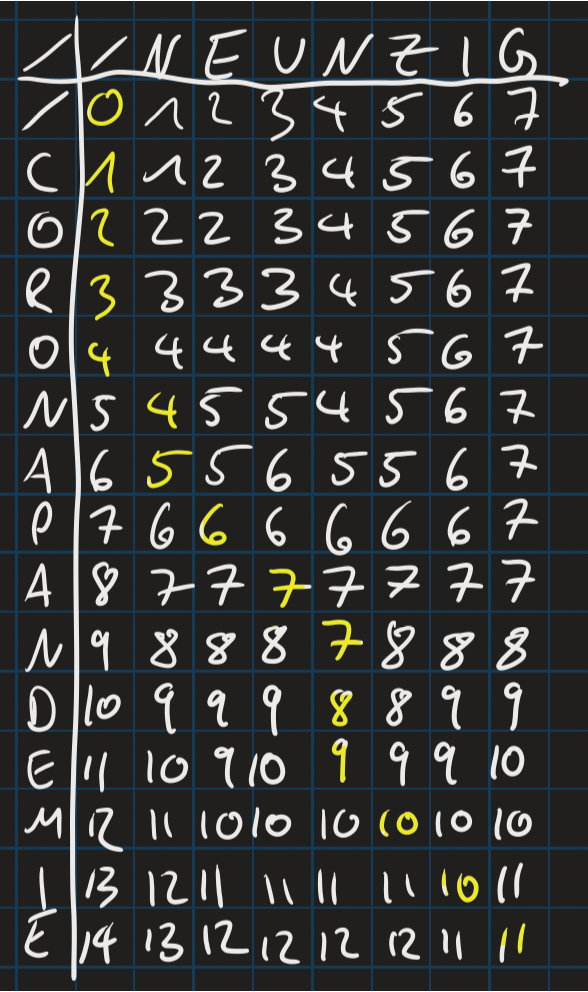
\includegraphics[width=0.4\textwidth]{Bilder/MatrixNormal.png} 
	\caption{Levenshtein-Matrix}
	\label{fig:matrix1}
\end{figure}

\section{Levenshtein Distanz}
\begin{quote}
    Aufbauend auf (a), wie hoch ist die Levenshtein similarity? (siehe Vorlesungsskript)
\end{quote}
Die Levenshtein-Similarity zwischen den Worten ''Coronapandemie'' und ''Neunzig'' liegt zwischen 1 und 0, wobei 1 heißt, dass die beiden Wörter gleich sind. Dadurch lässt sich die Similarity wie folgt berechnen: 
\begin{align*}
    1 - \frac{D}{L}
\end{align*}

$D$: Distanz

$L$: Länge des längsten Wortes

Aus (a) ist die Distanz bekannt. Wird die Distanz sowie die Länge des längsten Wortes (in diesem Fall ''Coronapandemie'') in die Formel eingesetzt, kann die Similarity nun berechnet werden:
\begin{align*}
    1 - \frac{11}{14} = 0,214
\end{align*}

Somit beträgt die Similarity zwischen den beiden Wörtern 0,214 oder 21,4\%

\section{Levenshtein Matrix mit unterschiedlichen Kosten}
\begin{quote}
    In (a) haben wir implizit für das Ersetzen, Hinzufügen und Löschen von Buchstaben Kosten von 1 angenommen. Jetzt ändern wir die Kosten für das Ersetzen eines Buchstabens zu 2. Die Kosten für das Hinzufügen und Löschen bleiben bei 1. Berechne erneut die Levenshtein Distanz des Wortes ''Coronapandemie'' zu deinem Nachnamen mit Hilfe der in der Vorlesung gezeigten Matrix-Methode
\end{quote}
Wenn für das Ersetzen eines Buchstaben Kosten von 2 anfallen, beträgt die Distanz 15. Die Matrix befindet sich in Abbildung \ref{fig:matrix2}.

\clearpage

\begin{figure}[ht]
	\centering
	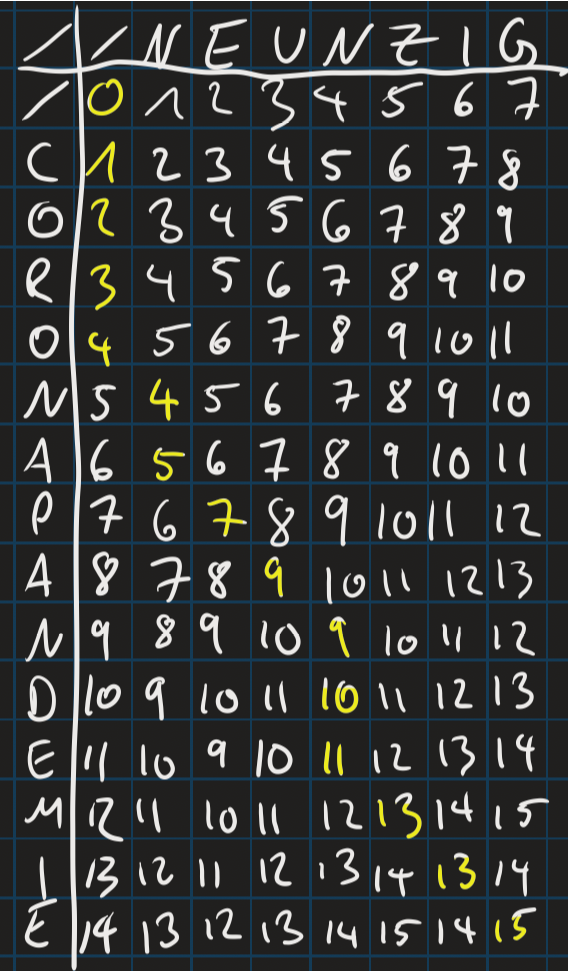
\includegraphics[width=0.4\textwidth]{Bilder/MatrixKosten.png} 
	\caption{Levenshtein-Matrix mit anderen Kosten}
	\label{fig:matrix2}
\end{figure}

\section{Jaccard Distanz}
\begin{quote}
    Berechne die Jaccard similarity des Wortes ''Coronapandemie'' zu deinem Nachnamen auf Basis von 2-grams. Liste dabei auch die jeweiligen 2-grams auf.
\end{quote}
Die Jaccard-Similarity der Wörter beträgt 0. Dies liegt daran, dass es keine übereinstimmenden 2-grams in den jeweiligen Mengen der beiden Wörter gibt: $A \cap B = 0$. Die 2-grams der Wörter ''Neunzig'' und ''Coronapandemie'' lauten wie folgt:

$A = \{NE, EU, UN, NZ, ZI, IG\}$

$B = \{CO, OR, RO, ON, NA, AP, PA, AN, ND, DE, EM, MI, IE\}$


